\chapter{Mediul Fizic}
Algoritmul genetic isi va optimiza problema in functie de mediul fizic oferit. Asta inseamna ca putem simula orice conditii fizice atat timp cat le putem reproduce. In cazul curent a fost simulat un mediu terestru cu $g = 9.8 m/s$. Mediul fizic incearca sa aproximeze fenomene fizice naturale folosind formule matematice.

\section{Integrarea ecuatiilor miscarii dupa dt}

Stiind ca $F=ma$ atunci putem scoate acceleratia unui obiect in functie de masa acestuia: $a = F/m$. Daca integram dupa timp atunci $dv/dt = a$ dar nu uitam ca $a=F/m$ deci putem spune ca viteza unui obiect va fi rata de schimbare a pozitiei acestuia in functie de timp $dx/dt = v$.

Punand tot cap la cap obtinem:
\begin{center}
    $a = F / m$\linebreak
    $dv = a * dt$\linebreak
    $dx = dv * dt$\linebreak
\end{center}

Deci daca vrem sa obtinem pozitia unui obiect dupa un anumit $dt$ vom calcula in urmatorul mod:
\begin{center}
    $a = F / m$\linebreak
    $v = v + a * dt$\linebreak
    $pos = pos + v * dt$\linebreak
\end{center}

Acesta este modul de integrare Semi-Implicit Euler.

\subsection{Moduri de integrare}
Exista mai multe moduri te integrare, cel prezentat mai sus este Semi-Implicit Euler.

Explicit euler integreaza pozitia inaintea vitezei si anume: 
\begin{center}
    $dx = dv * dt$\linebreak
    $a = F / m$\linebreak
    $dv = a * dt$\linebreak
\end{center}

Astfel apare o eroare in integrarea vitezei, iar aceasta depinde de timp. De exemplu aplicam o forta $F= 10N$ asupra unui corp de masa m, $m = 1kg$ timp de 10 secunde ($t = 10s$). Folosind formula miscarii uniforme $x = x_{0} + v_{0}t + \frac{at^{2}}{2}$ atunci $x = 500$, deci conform formulei, corpul se va misca 500 de unitati. Rezultatele integratorilor difera si anume:

Eroarea integratorului Explicit Euler creste in functie de $dt$ ales. Pentru $dt = 1.0$:
\begin{center}
    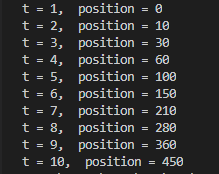
\includegraphics[width=0.3\textwidth]{explicit_euler_dt1.png}
\end{center}
La fel si pentru Semi-Implicit Euler
\begin{center}
    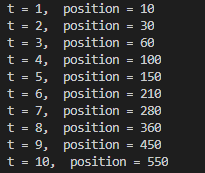
\includegraphics[width=0.3\textwidth]{semi-implicit_euler_dt1.png}
\end{center}

Se observa ca ambele integratoarea au acelasi grad de eroare, dar Semi-Implicit euler are o eroare in fata, comparat cu rezultatul cautat $x=500$ in timp ce Explicit-Euler este in urma. Eroare ambelor integratoare scade in functie de $dt$, si anume pentru $dt=0.5$ si $dt=0.016$ (timpul unui frame pentru on monitor cu o rata de reimprospatare de 60\textit{Hz}):
\begin{center}
    \textbf{Explicit Euler, dt=0.5 \& dt = 0.016}\linebreak
    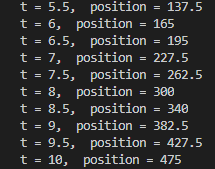
\includegraphics[width=0.3\textwidth]{explicit_euler_dt05.png}
    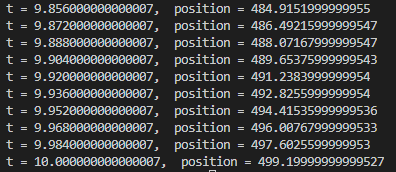
\includegraphics[width=0.545\textwidth]{explicit_euler_dt0016.png}
\end{center}
\begin{center}
    \textbf{Semi-Implicit Euler, dt=0.5 \& dt = 0.016}\linebreak
    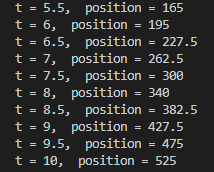
\includegraphics[width=0.3\textwidth]{semi-implicit_euler_dt05.png}
    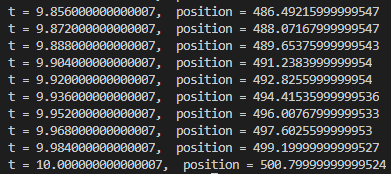
\includegraphics[width=0.545\textwidth]{semi-implicit_euler_dt0016.png}
\end{center}

Pentru $dt=0.016$ integratorul Semi-Implicit Euler obtine o eroare $\epsilon = 0.79$ iar integratorul Explicit Euler $\epsilon = 0.81$, deci Semi-Implicit Euler este mai bun cu $\epsilon = 0.02$ fara nici un cost suplimentar din punct de vedere al timpului de calcul sau a memoriei folosite.
\section{Rigid Bodies}
Un corp rigid este un corp ce nu sufera deformatii in niciul fel. In cadrul algoritmului genetic si a mediului fizic, orice obiect este considerat un corp rigid cu un anumit factor de elasticitate $\sigma \in [0,0.7]$. Avand in considerare scopul curent al algoritmului genetic, au fost alese cuburi cu $l = 1$. 

\section{Coliziuni}

Din moment ce calcularea fitnessului are loc in mediul fizic, este nevoie ca simularea sa se efectueze cat mai repede, astfel se va recurge la verificarea coliziunii in 2 faze.
\subsection{Intersectie intre doua sfere}
Primul pas in detectarea unei coliziuni va fi compararea intre 2 sfere $S1,S2$ ce se realizeaza in mod rapid:

\begin{center}
\textit{if} $d(C_{S1},C_{S2}) < (r_{S1}+r_{S2})$ \textit{then further checks... else false}
\end{center}

Fiecare obiect va fi invelit intr-o sfera de raza r:
\begin{center}
$r = d_{max}((0,0),v)$ unde $v \in Vertexes$. 
\end{center}

Astfel la fiecare frame, este necesar in prima faza doar o verificare de coliziune intre sfere, fapt care salveaza mult timp.

\begin{center}
    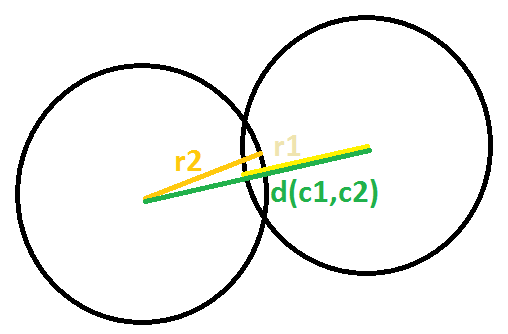
\includegraphics[width=0.5\textwidth]{sphere_colission.png} \linebreak
    \textit{exemplu coliziune intre 2 sfere}
\end{center}

\subsection{Intersectie intre doua triunghiuri}
Odata trecut cazul intersectiei intre doua sfere, pasul urmatorul este cautarea unui punct de intersectie intre triunghiurile obiectelor. Acest lucru se realizarea prin verificarea intersectiei dintre doua triunghiuri pentru toate perechile a cate doua triunghiuri dintre cele doua obiecte.

Articolul \textbf{A Fast Triangle-Triangle Intersection Test} \footnote{\url{http://web.stanford.edu/class/cs277/resources/papers/Moller1997b.pdf}} prezinta un mod optimizat de a realiza testul de intersectie si a fost folosit in cadrul implementarii.

\section{Efectul unei coliziuni}

In cazul nostru, coliziunile au loc doar intre indivizi si corpuri imobile. Astfel s-a folosit un mod simplu de impuls linear.

\begin{center}
    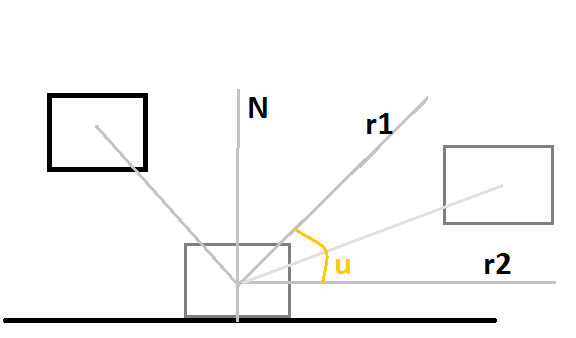
\includegraphics[width=0.5\textwidth]{colission_model.png}
\end{center}

Normala la contact $N$ se calculeaza din coordinatele varfurilor. Pentru un triunghi $T(p_{1},p_{2},p_{3})$ unde $p_{0},p_{1},p_{2}$ sunt varfurile de forma $p(x,y,z)$, atunci 
\begin{center}
    $N = (p_{1}-p_{0}) \times (p_{2}-p_{0})$
\end{center}

In functie de coeficientul de elasticitate $\mu$ al corpului, vectorul directie rezultat in urma coliziunii va fi intre $[r1,r2]$.
\begin{itemize}
    \item $\mu = 1$. Are loc o coliziune perfect elastica, fara pierdere de energie. Vectorul rezultat este r1. Acest caz a fost eliminat din algoritmul genetic.
    \item $\mu \in [0.9,0)$. Are loc o coliziune inelastica, o parte din energia cinetica este pierduta. Vectorul rezultat va fi intre $[r1,r2]$.
    \item $\mu = 0$. Are loc o coliziune perfect inelastica, obiectul va urma directia $r2$.
\end{itemize}